\section{Uninformed Orderflow's Value to LPs} \label{section:lp-oflow-value}
Before determining the value that uninformed orderflow creates for the protocol, we begin with the simpler problem of determining the value that it creates for Uniswap LPs. We present two lower bounds on this value. The first lower bound only counts the value created by an uninformed order itself, and the second lower bound counts the value created by sandwich attacks that are caused by uninformed orders.
    
\subsection{Lower Bound I: Uninformed Orderflow's Direct Value to LPs}
    How much value does an uninformed order create for Uniswap LPs?
    % We can start by defining the \textit{amountIn} vector of $\textbf a  = [a_0, a_1]^\text T$ to represent the amount in of the pool's token0 and token1, which has units of the respective tokens. 
    We define the \textit{token0 volume} of a transaction as $||\textbf a|| = \text{abs}(a_0)$, which has units of token0. Let $\gamma \in (0,1)$ be the fee paid by the trader, $\phi \in \{0, 1/4, 1/5, \dots, 1/9, 1/10 \}$ be the protocol fee. Let the price of the pool at time $t$ be $P_t$, and let the true price of token0 relative to token1 follow a random continuous-time stochastic process $S_t$. To find how much LPs should value this orderflow, we utilize the markout metric.

    \begin{definition}[$h$-Markout]
        For a given time lag $h$ and trade $\textbf{a}$ at time $t$, we define the markout for the order $\textbf{a}$ as 
        $$m_{\textbf{a}} = d \cdot ||\textbf{a}|| \cdot (P_{t + h} - \overline p(\textbf{a})),$$
        where $d$ is $-1$ if the LPs are selling token0 and $1$ if the LPs are buying token0, and $\bar p(\bf a)$ is the execution price of order $\bf a$, including fees paid to the LP.
    \end{definition}

    Markout embodies the quality of a trade, from the perspective of a market maker, of a trade placed at time $t$ and measured at a time $t+h$ in the future. While a positive value of markout does not imply that an LP's position is profitable long-term, it \textit{does} imply that the LP's trade is profitable at the time $h$ after the trade; a similar statement can be made for negative markout trades. However, this is not a critical flaw to the metric, for the following reason. If we assume that prices follow a zero-drift geometric Brownian motion (GBM), with no mean-reversion terms, then we can also demonstrate that for any lag $h' > h$, $$\mathbb E[\text{markout at time } t + h'] = \text{profit at time } t+h = m_\textbf{a}.$$ % TODO demonstrate that this is true
    This follows from the fact that the markout is simply a scalar addition and multiplication of the underlying price process $P_t$, and if $P_t$ follows a zero-drift GBM for times greater than $t+h$, our $h$-markout is the the same in expectation as $h'$ markout. In fact, it is not even necessary that $P_t$ follow a GBM; any continuous-time stochastic process $P_t$ that obeys $\mathbb E[P_{t+h'}] = \mathbb E[R_{t+h}]$ for any $h' > h$ suffices for markout to be equal in expectation at and after the lag-time $h$.

    Since this relationship often holds empirically, we find it to be an the most practical metric for measuring the value of an order for Uniswap LPs.

    % When the LP is selling token0 ($d=-1$), we have
    % $$\bar p(\textbf{a}) = \frac{y_{intoAmm} \cdot (1-\gamma\phi)}{x_{outOfAmm}} = \frac{(y_{reserveChange}/(1-\gamma)) \cdot (1-\gamma \phi)}{x_{reserveChange}} = \frac{1-\gamma\phi}{1-\gamma} \cdot p_{avgPostFee},$$

    % where $p_{traderAvgExec}$ is the average execution price for the trader, including the trader's fees paid. This gives us the following markout:
    % \begin{align*}
    %     m_{\textbf a} 
    %         & = (-1) \cdot ||\textbf{a}|| \cdot (S_{t+h} - \frac{1-\gamma\phi}{1-\gamma} \cdot p_{avgPostFee}) \\
    %         & = ||\textbf{a}|| \cdot (- S_{t+h} + \frac{1-\gamma\phi}{1-\gamma} \cdot p_{avgPostFee}) \\
    %         & \approx ||\textbf{a}|| \cdot (- S_{t+h} + (1 + (1-\phi)\gamma) \cdot p_{avgPostFee}) \\
    %         & = ||\textbf{a}|| \cdot p_{avgPostFee} \cdot \left( \gamma - \gamma \phi + \frac{p_{avgPostFee} - S_{t+h}}{p_{avgPostFee}} \right),
    % \end{align*}
    % using the Taylor approximation of $\frac{1-\gamma \phi}{1-\gamma}$ around $\gamma=0$ for the approximate-equal step.

    % A similar relationship holds when the LP is buying token0 ($d=1$):
    % \begin{align*}
    %     \bar p(\textbf{a}) 
    %         & = \frac{y_{outOfAmm}}{x_{intoAmm} \cdot (1-\gamma\phi)} = \frac{y_{reserveChange}}{(x_{reserveChange}/(1-\gamma)) \cdot (1-\gamma\phi)} \\
    %         & = \frac{1-\gamma}{1-\gamma\phi} p_{avgPostFee}, \text{ and} \\
    %     m_\textbf{a} 
    %     & = ||\textbf a|| \cdot (S_{t + h} - \frac{1-\gamma}{1-\gamma\phi} p_{avgPostFee}) \\
    %     & \approx ||\textbf a|| \cdot (S_{t + h} - (1 - \gamma + \gamma\phi) p_{avgPostFee}) \\
    %     & = ||\textbf a|| \cdot p_{avgPostFee} \cdot \left( \gamma - \gamma\phi + \frac{S_{t + h} - p_{avgPostFee}}{p_{avgPostFee}} \right).
    % \end{align*}

    % Notice that these markout derivations work for both Uniswap V2 and Uniswap V3, since each AMM utilizes a $\gamma$ fee on input and $\phi$ protocol fee.

    \begin{theorem}[Expected markout on a single uninformed order]
        Given an order $\textbf a$, its expected markout for LPs, $\mathbb E[m_{\textbf a}]$, is lower bounded by the fees that LPs earn on the order. That is,
            $$\mathbb E[m_{\textbf a}] > || \textbf a || \cdot p_{avgPostFee} \cdot (\gamma(1-\phi)).$$
    \end{theorem}

    \begin{proof}
        We begin by obtaining an expression for $\overline p(\textbf{a})$, where $x$ represents an amount of token0 and $y$ represents an amount of token1.

            $$\bar p(\textbf{a}) = \frac{y_{intoAmm} \cdot (1-\gamma\phi)}{x_{outOfAmm}} = \frac{(y_{reserveChange}/(1-\gamma)) \cdot (1-\gamma \phi)}{x_{reserveChange}} = \frac{1-\gamma\phi}{1-\gamma} \cdot p_{avgPostFee}.$$
        
        This allows us to represent markout in the following way
        \begin{align*}
            m_{\textbf a} 
                & = (-1) \cdot ||\textbf{a}|| \cdot (S_{t+h} - \frac{1-\gamma\phi}{1-\gamma} \cdot p_{avgPostFee}) \\
                & = ||\textbf{a}|| \cdot (- S_{t+h} + \frac{1-\gamma\phi}{1-\gamma} \cdot p_{avgPostFee}) \\
                & \approx ||\textbf{a}|| \cdot (- S_{t+h} + (1 + (1-\phi)\gamma) \cdot p_{avgPostFee}) \\
                & = ||\textbf{a}|| \cdot p_{avgPostFee} \cdot \left( \gamma - \gamma \phi + \frac{p_{avgPostFee} - S_{t+h}}{p_{avgPostFee}} \right),
        \end{align*}
        using the Taylor approximation of $\frac{1-\gamma \phi}{1-\gamma}$ around $\gamma=0$ for the approximate-equal step.

        With this definition for markout, we may now move on to determining the value that an uninformed order $\textbf{a}$ would create for the LPs of a pool. When $d=-1$, we would have
        \begin{align*}
            \mathbb E[m_\textbf a] 
                & = \mathbb E \left[
                    ||\textbf{a}|| \cdot p_{avgPostFee} \cdot \left( \gamma - \gamma \phi + \frac{p_{avgPostFee} - S_{h}}{p_{avgPostFee}} \right) \ | \ \textbf a \ 
                \right] \\
                & = ||\textbf{a}|| \cdot p_{avgPostFee} \cdot \left( \gamma - \gamma \phi + \frac{p_{avgPostFee} - \mathbb E \left[S_{h} \ | \ \textbf a \right]}{p_{avgPostFee}} \right).
        \end{align*}

        Now we assume that $\mathbb E[S_{h} \ | \ \textbf a] = \mathbb E[P_{h} \ | \ \textbf a]$; this assumption should intuitively follow from the existence of arbitrage for sufficiently large $h$. This gives us the following
            \begin{align*}
                \mathbb E[m_\textbf a]
                    & = ||\textbf{a}|| \cdot p_{avgPostFee} \cdot \left( \gamma - \gamma \phi + \frac{p_{avgPostFee} - \mathbb E \left[S_{h} \ | \ \textbf a \right]}{p_{avgPostFee}} \right) \\
                    & = ||\textbf{a}|| \cdot p_{avgPostFee} \cdot \left( \gamma - \gamma \phi + \frac{p_{avgPostFee} - \mathbb E \left[P_{h} \ | \ \textbf a \right]}{p_{avgPostFee}} \right).
            \end{align*}
    
        Now, if we assume that an order is $h$-uninformed, it follows that $\mathbb E[P_{t} \ | \ \textbf a] = E[P_{t+h}]$, and we find that
            \begin{align*}
                \mathbb E[m_\textbf a]
                    & = ||\textbf{a}|| \cdot p_{avgPostFee} \cdot \left( \gamma - \gamma \phi + \frac{p_{avgPostFee} - \mathbb E \left[P_{h} \ | \ \textbf a \right]}{p_{avgPostFee}} \right) \\
                    & = ||\textbf{a}|| \cdot p_{avgPostFee} \cdot \left( \gamma - \gamma \phi + \frac{p_{avgPostFee} - \mathbb E \left[ P_{h} \right]}{p_{avgPostFee}} \right).
            \end{align*}

        If we assume that $\mathbb E[P_{t+h}] = P_t$, then we find 
            \begin{align*}
                \mathbb E[m_\textbf a]
                    & = ||\textbf{a}|| \cdot p_{avgPostFee} \cdot \left( \gamma - \gamma \phi + \frac{p_{avgPostFee} - \mathbb E \left[ P_{h} \right]}{p_{avgPostFee}} \right) \\
                    & = ||\textbf{a}|| \cdot p_{avgPostFee} \cdot \left( \gamma - \gamma \phi + \frac{p_{avgPostFee} - p_0}{p_{avgPostFee}} \right) \\
                    & > ||\textbf{a}|| \cdot p_{avgPostFee} \cdot (\gamma(1-\phi)).
            \end{align*}

        This demonstrates the desired result for $d=-1$, the case where the pool is selling token0. A similar result can be shown for the case of $d=1$.
    \end{proof}

    Despite the legwork required for the proof, this result should be rather intuitive: in expectation, Uniswap LPs make at least the LP fee on each unit of uninformed volume in the pool. Technically, LPs make slightly more that this value in expectation, due to the fact that uninformed orders move the pool price. Although this approach has given us a lower bound on the $h$-markout of an uninformed order, it ignores the $h$-markout of other orders that are caused by uninformed orders. In particular, the uninformed order $h$-markout ignores sandwich volume. We now create another lower bound on markout value that takes sandwich attacks into account.
        
    %     \begin{align*}
    %         \mathbb E[m_\textbf a] 
    %             & = \mathbb E \left[ (-1) \cdot ||\textbf a|| \cdot (S_{h} - \bar p(\textbf a)) \right] \\
    %             & = (-1) \cdot ||\textbf a|| \cdot (\mathbb E [S_{h} \ | \ \textbf a] - \bar p(\textbf a)).
    %     \end{align*}
    
    % Then, if we assume that price discovery being independent of Uniswap trades, we have that
    %     \begin{align*}
    %         \mathbb E[m_\textbf a] 
    %             & = (-1) \cdot ||\textbf a|| \cdot (\mathbb E [S_{h} \ | \ \textbf a] - \bar p(\textbf a)) \\
    %             & = (-1) \cdot ||\textbf a|| \cdot (\mathbb E [S_{h}] - \bar p(\textbf a)).
    %     \end{align*}
    
    % Next, we assume that the $\mathbb E [S_0] = \mathbb E [S_{h}]$. This assumption is akin to a zero-drift assumption when modelling prices as a geometric brownian motion. This gives us
    %     \begin{align*}
    %         \mathbb E[m_\textbf a] 
    %             & = (-1) \cdot ||\textbf a|| \cdot (\mathbb E [S_{h}] - \bar p(\textbf a)) \\
    %             & = (-1) \cdot ||\textbf a|| \cdot (S_0 - \bar p(\textbf a)).
    %     \end{align*}

    % Now we use our derivation of $\bar p(\textbf a)$ from above to get
    %     \begin{align*}
    %         \mathbb E[m_\textbf a] 
    %         & = (-1) \cdot ||\textbf a|| \cdot (\mathbb E [S_{h}] - \bar p(\textbf a)) \\
    %         & = (-1) \cdot ||\textbf a|| \cdot (S_0 - \bar p(\textbf a)) \\
    %     \end{align*}

        

    % \begin{align}
    %     \mathbb E[m_\textbf a] 
    %         & = \mathbb E \left[ (-1) \cdot ||\textbf a|| \cdot (S_{t + h} - \bar p(\textbf a)) \right] \\
    %         & = (-1) \cdot ||\textbf a|| \cdot (\mathbb E [S_{t + h} \ | \ \textbf a] - \bar p(\textbf a)) \\
    %         & = (-1) \cdot ||\textbf a|| \cdot (\mathbb E [S_{t + h}] - \bar p(\textbf a)) \\
    %         & = (-1) \cdot ||\textbf a|| \cdot (\mathbb E [S_0] \cdot e^{\mu \cdot h} - \bar p(\textbf a)) \\
    %         & = ||\textbf a|| \cdot (\bar p(\textbf a) - p_0 \cdot e^{\mu \cdot h}) \\
    %         & = ||\textbf a|| \cdot (\bar p(\textbf a) - p_0) \\
    %         & = ||\textbf a|| \cdot (\frac{1}{1-\gamma} \cdot p_{avgExecPricePostFee} - p_0) \\
    %         & > ||\textbf a|| \cdot ((1+\gamma) \cdot p_0 - p_0) \\
    %         & = ||\textbf a|| \cdot (\gamma \cdot p_0).
    % \end{align}


\subsection{Lower Bound II: Uninformed Orderflow's Sandwich Value to LPs} \label{subsection:sandwich-value-to-lps}
    We have demonstrated, for a given order, a lower bound on the LPs' expected markout. Interestingly, some uninformed orders can \textit{cause} other orders, and in this case, we should ascribe the value of the \textit{caused} order to the uninformed order that caused it. This is far more than a theoretical distinction, since it occurs in real life in the form of sandwich attacks.

    A sandwich attack is a type of economic attack that occur on blockchains that propagate trades via public mempools, such as is the case for orders placed on Ethereum Mainnet through the \texttt{app.uniswap.org} trading interface. If a trader \textit{Alicia} specifies a worst-case execution price that is far worse than the price she would get from trading on the last block's state, then it is possible for another trader, Bobby, to place an order before the Alice's order and after Alice's order  to ``sandwich'' the her order. Henceforth, we refer to Bobby's first and second transaction as the front- and back-run transactions, respectively; we will refer to Alice's transaction as the victim transaction. There is extensive literature on sandwich attacks and their mitigations (\cite{kulkarni2022towards}, \cite{zust2021analyzing}, \cite{zhou2021high}).
    
    The reason sandwiches play a relevant role in this analysis is due to the fact that they are typically caused by an uninformed order, typically via unsophisticated users who place orders with sloppy slippage tolerance and broadcast these orders through public channels. Since the front- and back-run orders surrounding the uninformed victim order also must pay fees, it is clear that those orders also lead to similar fees paid to miners. We observe empirically that these front- and back-run orders are themselves balanced, selling the same amount as that which is purchased -- and thus do not demonstrate the directionality that would be needed in order for them to be predictive of future price movements. That is to say, front- and back-run orders appear to be uninformed, and thus they yield the same markout for LPs as regular uninformed orderflow.

    To find the amount of sandwich value that an uninformed order creates for LPs, we can utilize either of two orthogonal approaches: (a) demonstrate optimal sandwich sizes with respect to uninformed order size and slippage tolerance, and (b) use empirical data to find the amount of sandwich value that historical uninformed orders have created for LPs. We demonstrate both approaches here.

    \subsubsection{Quantifying Sandwich Value Analytically}
        For Uniswap V2, \cite{heimbach2022eliminating} derived the optimal sandwich size with respect to an uninformed order. The resulting analytical solution provides formulas for computing the optimal sandwich input amounts for the front- and back-running trades.

        For orders on Uniswap V2 that have no slippage tolerance specified and which is purchasing token1 (WOLOG), the optimal sandwich order input size is the following:

        \begin{equation*}
            \delta^o_{a_x} = 
                \frac{\delta_{v_x}(1-\gamma)^2x_0 - (2-\gamma)\gamma x_0^2}{(2-\gamma)\gamma x_0 - \delta_{v_x}(1-\gamma)^2\gamma} 
                + \frac{\sqrt{\delta_{v_x}^2 (1-\gamma)^3x_0(x_0-(1-\gamma)^2\gamma)}}{(2-\gamma)\gamma x_0 - \delta_{v_x}(1-\gamma)^2\gamma},
        \end{equation*}

        where $\delta^o_{a_x}$ is the optimal sandwich size, $\delta_{v_x}$ is the amount of token0 that the victim is putting into the AMM, and $x_0$ is the amount of token0 in the pool initially \cite{heimbach2022eliminating}. When an order specifies a slippage tolerance $s$, then the optimal sandwich amount is the following:
        \begin{equation*}
            \delta_{a_x}^s=\frac{\frac{\sqrt{n\left(x_0, \gamma, \delta_{v_x}, s\right)}}{1-s}-\delta_{v_x}(1-\gamma)^3-(2-\gamma)(1-\gamma) x_0}{2(1-\gamma)^2},
        \end{equation*}
        where
        \begin{align*}
            n\left(x_0, \gamma, \delta_{v_x}, s\right) = &  \ (1-\gamma)^2(1-s)\left(\delta_{v_x}^2(1-\gamma)^4(1-s)\right. 
             +2 \delta_{v_x}(1-\gamma)^2(2-\gamma(1-s)) x_0 \\
            & \ + (4-\gamma(4-\gamma(1-s))) x_0^2.
        \end{align*}
        
        For an algorithm on how we can utilize this method on Uniswap V3, see appendix \ref{appendix:opt-sandwich}.

        We can utilize these optimal sandwich order formulas, along with historical on-chain liquidity data, to find the amount that a sandwiched order $\textbf a$  would create for LPs, in effect allowing us to give a sandwich correction factor that we could add to our markout formula above. 

        % TODO expand on the methodology for utilizing optimal sandwich size to compute the markout value of sandwich volume

        Although this analytical-like method has an appeal, it still requires an algorithm to compute, it requires us to use historical on-chain liquidity data, and it requires us to make gas price assumptions. This makes the method most apt for \textit{ex ante} estimation of the value of uninformed orderflow. If we can wait to ascribe value to orderflow \textit{ex post}, then we can utilize the empirical approach below in section \ref{section:sandwich-value-empirical}.

    
    \subsubsection{Quantifying Sandwich Value Empirically} \label{section:sandwich-value-empirical}
    
        As an alternative to determining optimal sandwiching analytically, we can utilize historical sandwich data to measure the amount of value created for LPs as a result of an uninformed order getting sandwiched.

        \textbf{Data collection methodology}. 
        To collect this data, we use the Uniswap V3 subgraph, and the analysis presented here is performed specifically on the ETH-USDC 0.05\% fee Uniswap V3 pool. We check that a transaction is sandwiched by utilizing the same methodology as Johnny Chuang and Anderson Chen in their Uniswap bounty 
        \cite{chuang2022mev}. 
        We deem that an order $o$ has been sandwiched if the following conditions hold: (0) there is an address \textit{Addy} that placed two orders in the same block as $o$, (1) the orders on either side of $o$ were placed by \textit{Addy}, (2) \textit{Addy}'s order before $o$ was in the same direction as $o$, (3) \textit{Addy}'s order after \textit{o} was in the opposite direction as \textit{o}, (4) the orders on either side of \textit{Addy}'s order are do not utilize an aggregator or router contract, and (5) the orders on either side of \textit{Addy}'s have a token0 amount within 50\% of each other. We apply this filter to all of the swaps in all of the Ethereum blocks from July 31, 2022 - Dec 31, 2022 to create a dataset of sandwiches.

        \textbf{Results}.
        We find that sandwiched orders create an immense amount of value for the LPs of the protocol.
        The important figures can be found in appendix \ref{appendix:sandwich-data}, and we present some of the most important figures here.
        
        % We identified 3819 sandwich attacks between July 7, 2022 and January 2, 2022. Across all sandwich attacks, there was a cumulative \$11,496,000,000 in ``bun'' volume and \$2,051,000,000 in ``meat'' volume; put another way, for every dollar of meat volume, there were over \$5 of bun volume. All in all, this led to over \$5,700,000 in fees paid by sandwich bots to LPs, or 14\% of the total fees paid over that period.

        \begin{figure}
            \label{fig:meat-bun-ratio}
            \centering
            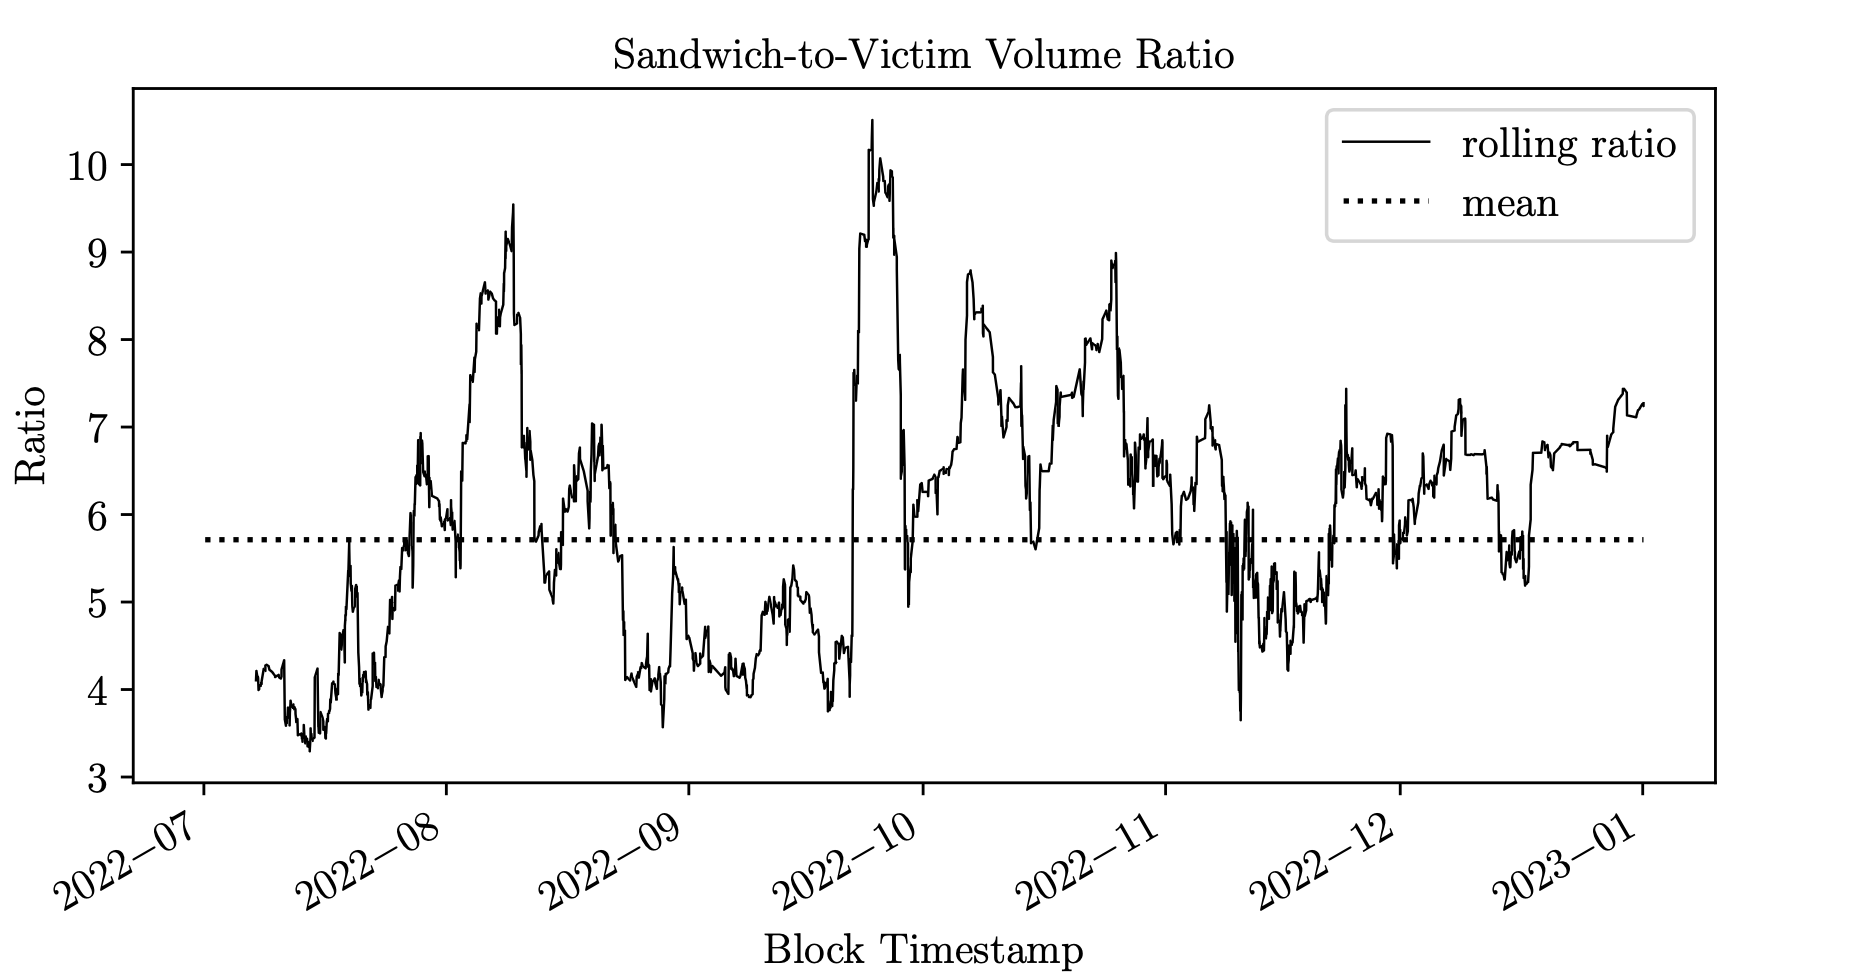
\includegraphics[scale=.4]{figs/bun-to-meat-ratio.png}
            \caption{The 100-sandwich rolling ratio of bun volume to meat volume for the ETH-USDC 0.05\% pool.}
        \end{figure}

        % TODO review this section once we verify the sandwich data
        We also present plot \ref{fig:meat-bun-pairplots}, showing the volume of the sandwich victim and front-/back-run orders. We see that there are two regions of sandwiches, with a cutoff at approximately 100,000 USDC of meat volume. Roughly speaking, when the meat volume is less than 100,000 USDC, the bun volume is correlated to the meat volume (left plot); when the meat volume is greater than 100,000 USDC, the bun volume is not correlated to the meat volume. This arises due to there being two regions of sandwich optimization. When the meat volume is less than small (e.g. less than 100,000 USDC) the sandwich bot must balance its LP fees paid vs its revenue from the sandwich attack. When the meat volume is large (e.g. greater than 100,000 USDC) the sandwich bot will place orders large enough to hit the meat order's maximum slippage.

        \begin{figure}
            \label{fig:meat-bun-pairplots}
            \centering
            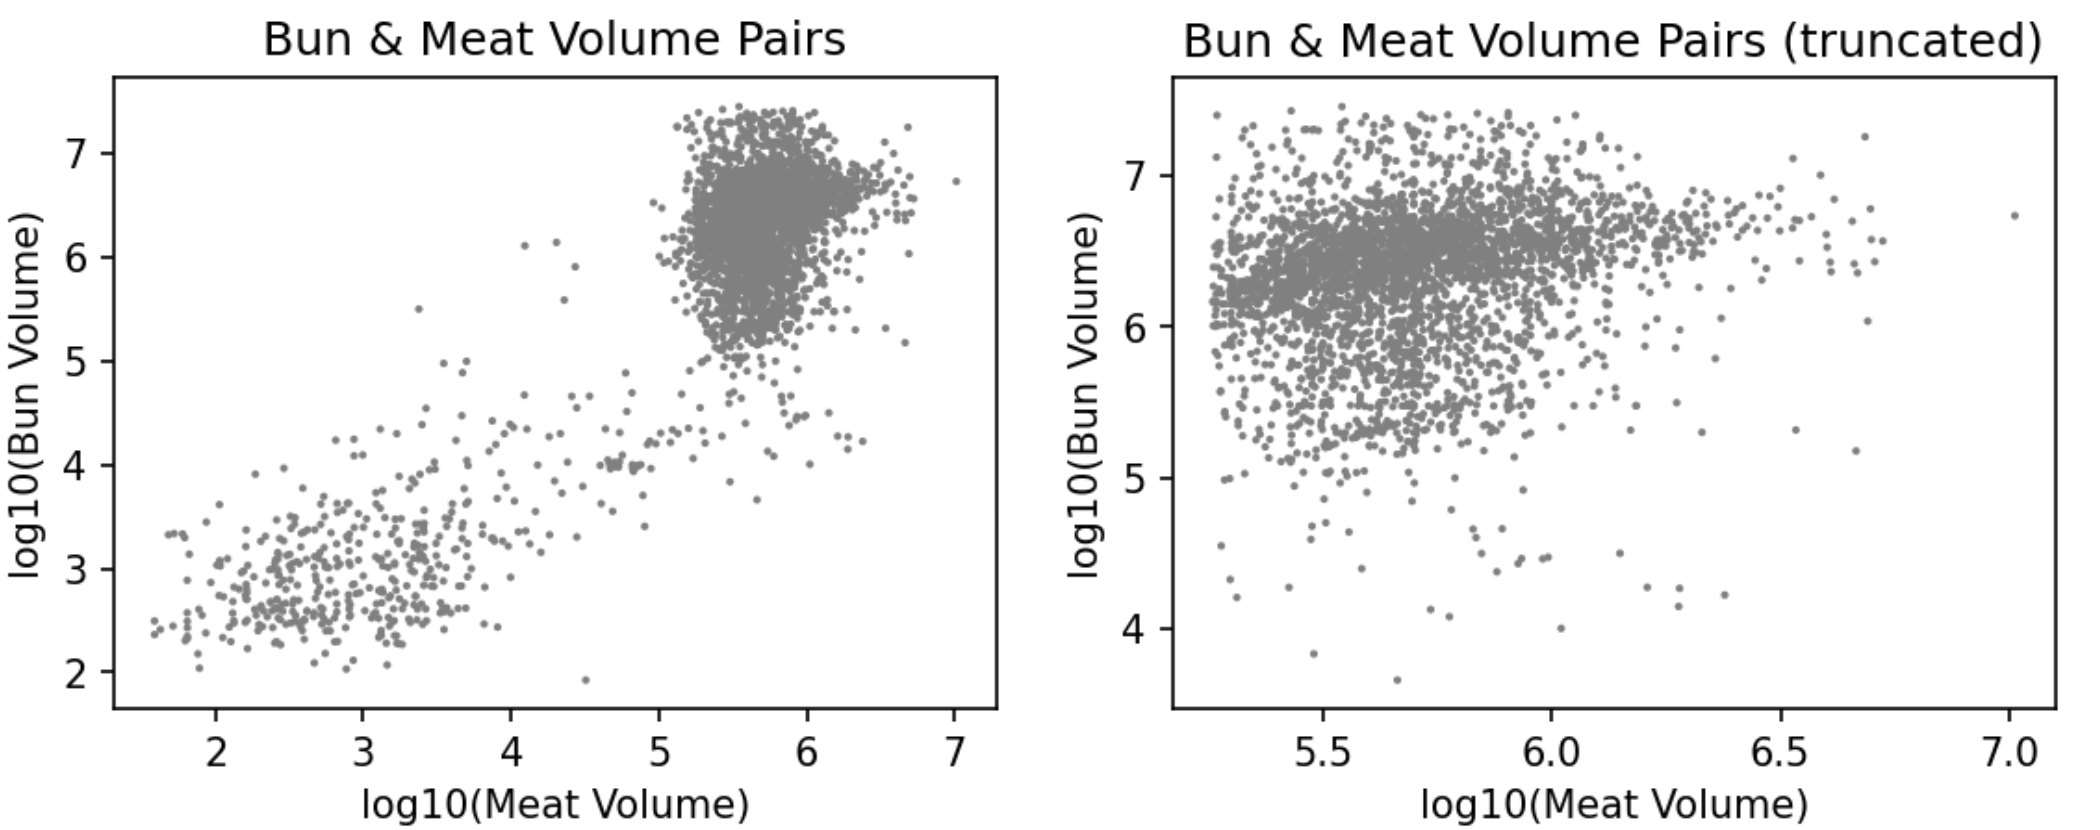
\includegraphics[scale=.43]{figs/meat-and-bun-pairwise-plot.png}
            \caption{Scatter plots of (meat, bun) volume pairs. The left plot shows all of the sandwich data, and the right plot only considers sandwiches where the meat volume is greater than 100,000 USDC.}
        \end{figure}

        \begin{figure}
            \label{fig:meat-bun-pairplot-small}
            \centering
            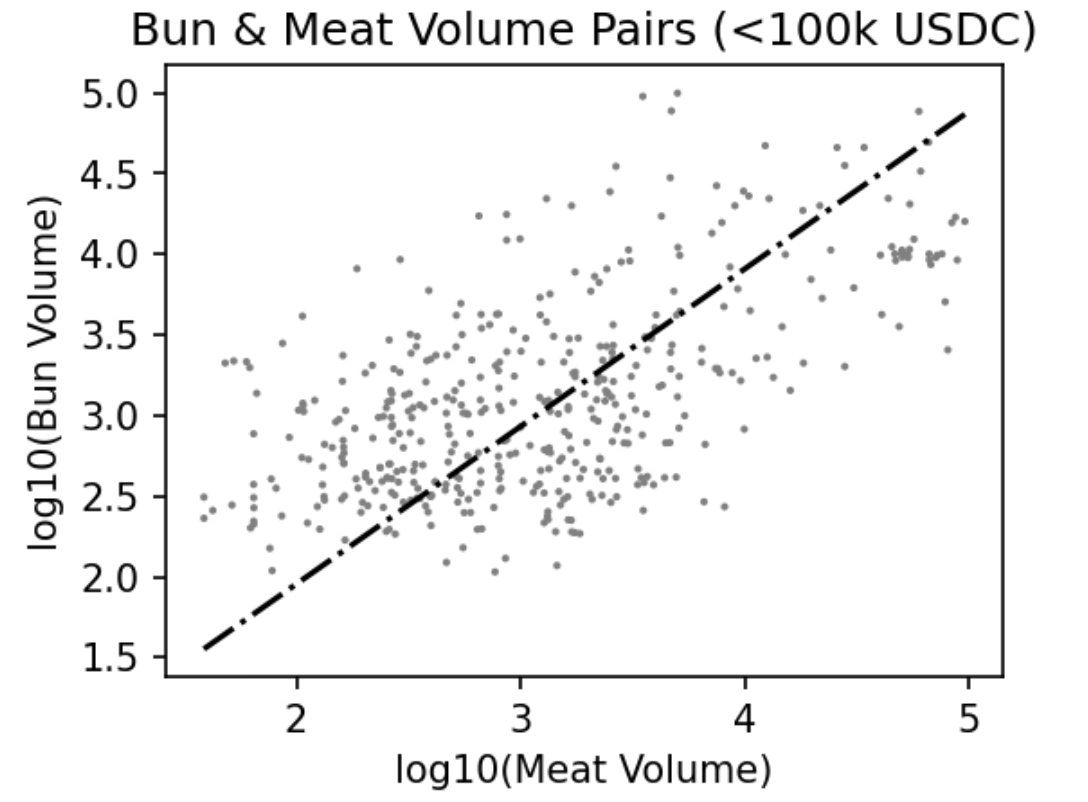
\includegraphics[scale=.43]{figs/meat-and-bun-pairwise-small-meat.png}
            \caption{Scatter plots and line of best fit for (meat, bun) volume pairs for meat volume less than 100,000 USDC.}
        \end{figure}
        

        By inspection, we can tell from these graphs that a sandwiched order of volume $10^{5.8}$ can realistically cause anywhere from 100,000 USDC to 10,000,000 USDC. Although we can approximate the amount of sandwich volume that a sandwiched order causes, the value varies widely, and we should not give a closed-form approximation of the value of sandwich fees generated from a single sandwiched order. Instead, it is more fair to say that, by inspection of the ratio plot \ref{fig:meat-bun-ratio}, on-average  victim volume causes between 4 and 7 times as much front- and back-run volume.












































%%%%%%%%%%%%%%%%%%%%%%%%%%%%%%%%%%%%%%%%%%%%%%%%%%%%%%%%%%%%%%%%%%%%%%%%%%%%%%%%%%%%%%%% OLD %%%%%%%%%%%%%%%%%%%%%%%%%%%%%%%%%%%%%%%%%%%%%%%%%%%%%%%%%%%%%%%%%%%%%%%%%%%%%%%%%%%%%%%%


% \section{Value of Uninformed Orderflow for LPs} \label{section:lp-oflow-value}
% We proceed with the following methodology to determine the revenue that uninformed orderflow creates for LPs in an Uniswap V3 pool.
% First, we use historical order data to filter orders into informed vs uninformed orders, and we estimate the distribution of sizes of uninformed orders.
% Next, we run a number of simulations in which we sample from this estimated distribution of uninformed order sizes and compute the amount of revenue generated to LPs from that uninformed order; this revenue quantity includes the revenue that would be generated by sandwiching the uninformed order. This allows us to both determine the value created by uninformed orders of various sizes and determine the mean value per dollar of uninformed orderflow.
% We then use these values to estimate the influx of LP positions that we would expect to see as a result of an increase in LP revenue. To do this, we use historical pool data to filter positions into \textit{active} and \textit{passive}, based on how long they have been open, and we assume that the active positions will behave more rationally with respect to increases in LP revenues, whereas we assume that passive positions will be less responsive. By doing this, we can place a conservative estimate on the influx of new LP positions that would result from an increase in LP revenues.

% \subsection{The distribution of uninformed order sizes.}
% % 1. We sample from historical Uniswap trades to find the distribution of uninformed orderflow sizes. We outline our methodology for determining which orders are informed in the appendix.
% We estimate the distribution of uninformed order sizes by filtering historical orders into informed and uninformed orders, then approximating the distribution of historical trade sizes. To perform this filtering, we


% \subsection{Simulating uninformed orderflow's impact on LP revenue.}
% % 2. We sample from these historical trades to find the liquidity present at the time those swaps are made. We can use this to fit a function from swap size -> liquidity, although that regression may not be necessary / have statistical significance.

% % 3. We run simulations whereby we sample a swap size, compute the amount of fees that it generates for the LPs, and find the amount of capital vs dollar of swap size.


% \subsection{Relating LP revenue to LP positions.}
% % 4. We then estimate the amount of additional liquidity we would expect in the pool, due to this increase in revenues. We do this in a rather unsophisticated way, by computing (new positions) = (new revenue)/(old revenue) * (old positions), and from this we could compute some liquidity metric L(new positions) and compare it to a liquidity metric L(old positions). However, this is almost certainly an over-estimation of the new liquidity, since it is unlikely that all of the original positions are linearly related to protocol revenues. 
% % 5. We could do something to estimate which capital is _sticky_ vs _not sticky_ by instead just looking at (old positions | position has existed over a shorter term). These actively-managed positions are more likely to be elastic to LP revenues, and presumably they are managed by "smart money" market makers who would increase their capital deployed if there was an opportunity to earn more revenue. This does add another parameter to our problem -- the cutoff for how long a position has existed -- but we can see how it varies and adjust to something that's reasonable. We'll provide a couple different params. We'll choose an aggressively short term filter for the positions, then compute (new active positions) = (new revenue)/(old revenue) * (old positions), then compute (new positions) = (old positions - old active positions + new active positions), then compute L(new positions). This is the most practical approach we could derive for estimating the increase in LPs. Assumptions. (1) Uniswap uninformed swap size distribution will be the same in the future as it is today, (2) this liquidity model is sufficient to capture liquidity, (3) more like a possible issue is that we're not measuring gains to passive liquidity, (4) ?
% % Another model for computing additional liquidity is to compute the PnL of LPing, see how this increases (in expectation) with more fee revenue, then see how you'd Markowitz-style optimize it, then see what the new liquidity positions would be. This would require an immense amount of assumptions though: uniform LP risk-reward preferences, uniform LP strategies, usage of a risk-free rate, etc.

